\label{chp:anharmonicity}

\REM{update intro when chapter is ready}

We have seen in the previous chapter that thermal conductivity is an anharmonic effect --- in a purely harmonic system, thermal conductivity is ill-defined. We have also discussed methods to assess vibrational thermal transport in materials from first principles: Either via the \emph{ab initio} Green-Kubo approach~\cite{Marcolongo.2016,Carbogno.2016}, or via perturbation theory, where the potential energy is expanded to third or fourth order in the atomic displacements, and these terms are used to compute the change of phonon properties such as their lifetimes~\cite{Broido.2007,Simoncelli.2019,Isaeva.2019,Feng.2016,Feng.2017,Ravichandran.2018,Xia.2018}.

As we will see, the discussion of the differences between these approaches will be greatly facilitated once we can formally define and assess ``anharmonicity'' in a quantitative way. To this end, we have developed a scheme to measure the strength of anharmonicity in a material by means of a single number,~$\sigmaA$, irrespective of physical observables.



\section{Definition of Anharmonicity}

In accordance with the previous chapters, classical nuclear dynamics within the Born-Oppenheimer approximation is governed by the Hamiltonian
\begin{align}
	\mathcal H ( {\bf P}, {\bf R}) 
		= \sum_I \frac{\b P_I^2}{2 M_I} + \mathcal V (\b R)~,
	\label{eq:anh.H}
\end{align}
where $\bf P$ and $\bf R$ denote the atomic momenta and coordinates. Using an expansion of the the full potential $\mathcal V ({\bf R})$ in the displacements $\bf U$ around a reference configuration ${\bf R}^0$ as discussed in Chp.\,\ref{chp:dynamics}, the potential can be split into a harmonic contribution, $\mathcal V^{(2)}$, and a second term capturing all anharmonic effects, $\mathcal V^{\rm A}$,
\begin{align}
	\mathcal V ({\bf R})
		= \mathcal V^{(2)} ({\bf R}) + \mathcal V^{\rm A} ({\bf R})~.
	\label{eq:anh.V}
\end{align}
In the classical limit, the dynamical evolution of the nuclei is determined by the potential through the interatomic forces as defined Eq.\,\eqref{eq:dyn.eom.classical},
\begin{align}
	M_I \ddot{\bf R}_I
		= -\frac{\partial \mathcal V}{\partial {\bf R}_I}
		\equiv {\bf F}_I~,
\end{align}
~i.\,e.,~Newton's equations of motion. By linearity of the differential, the forces can therefore be split into harmonic and anharmonic contributions as well,
\begin{align}
	{\bf F}_I
		= {\bf F}_I^{(2)} + {\bf F}_I^{\rm A}~.
	\label{eq:anh.F}
\end{align}
The division of potential and forces into harmonic and anharmonic contributions is depicted for a one-dimensional potential in Fig.\,\ref{fig:pes_sketch_vertical}.
\begin{marginfigure}
	\centering
	% 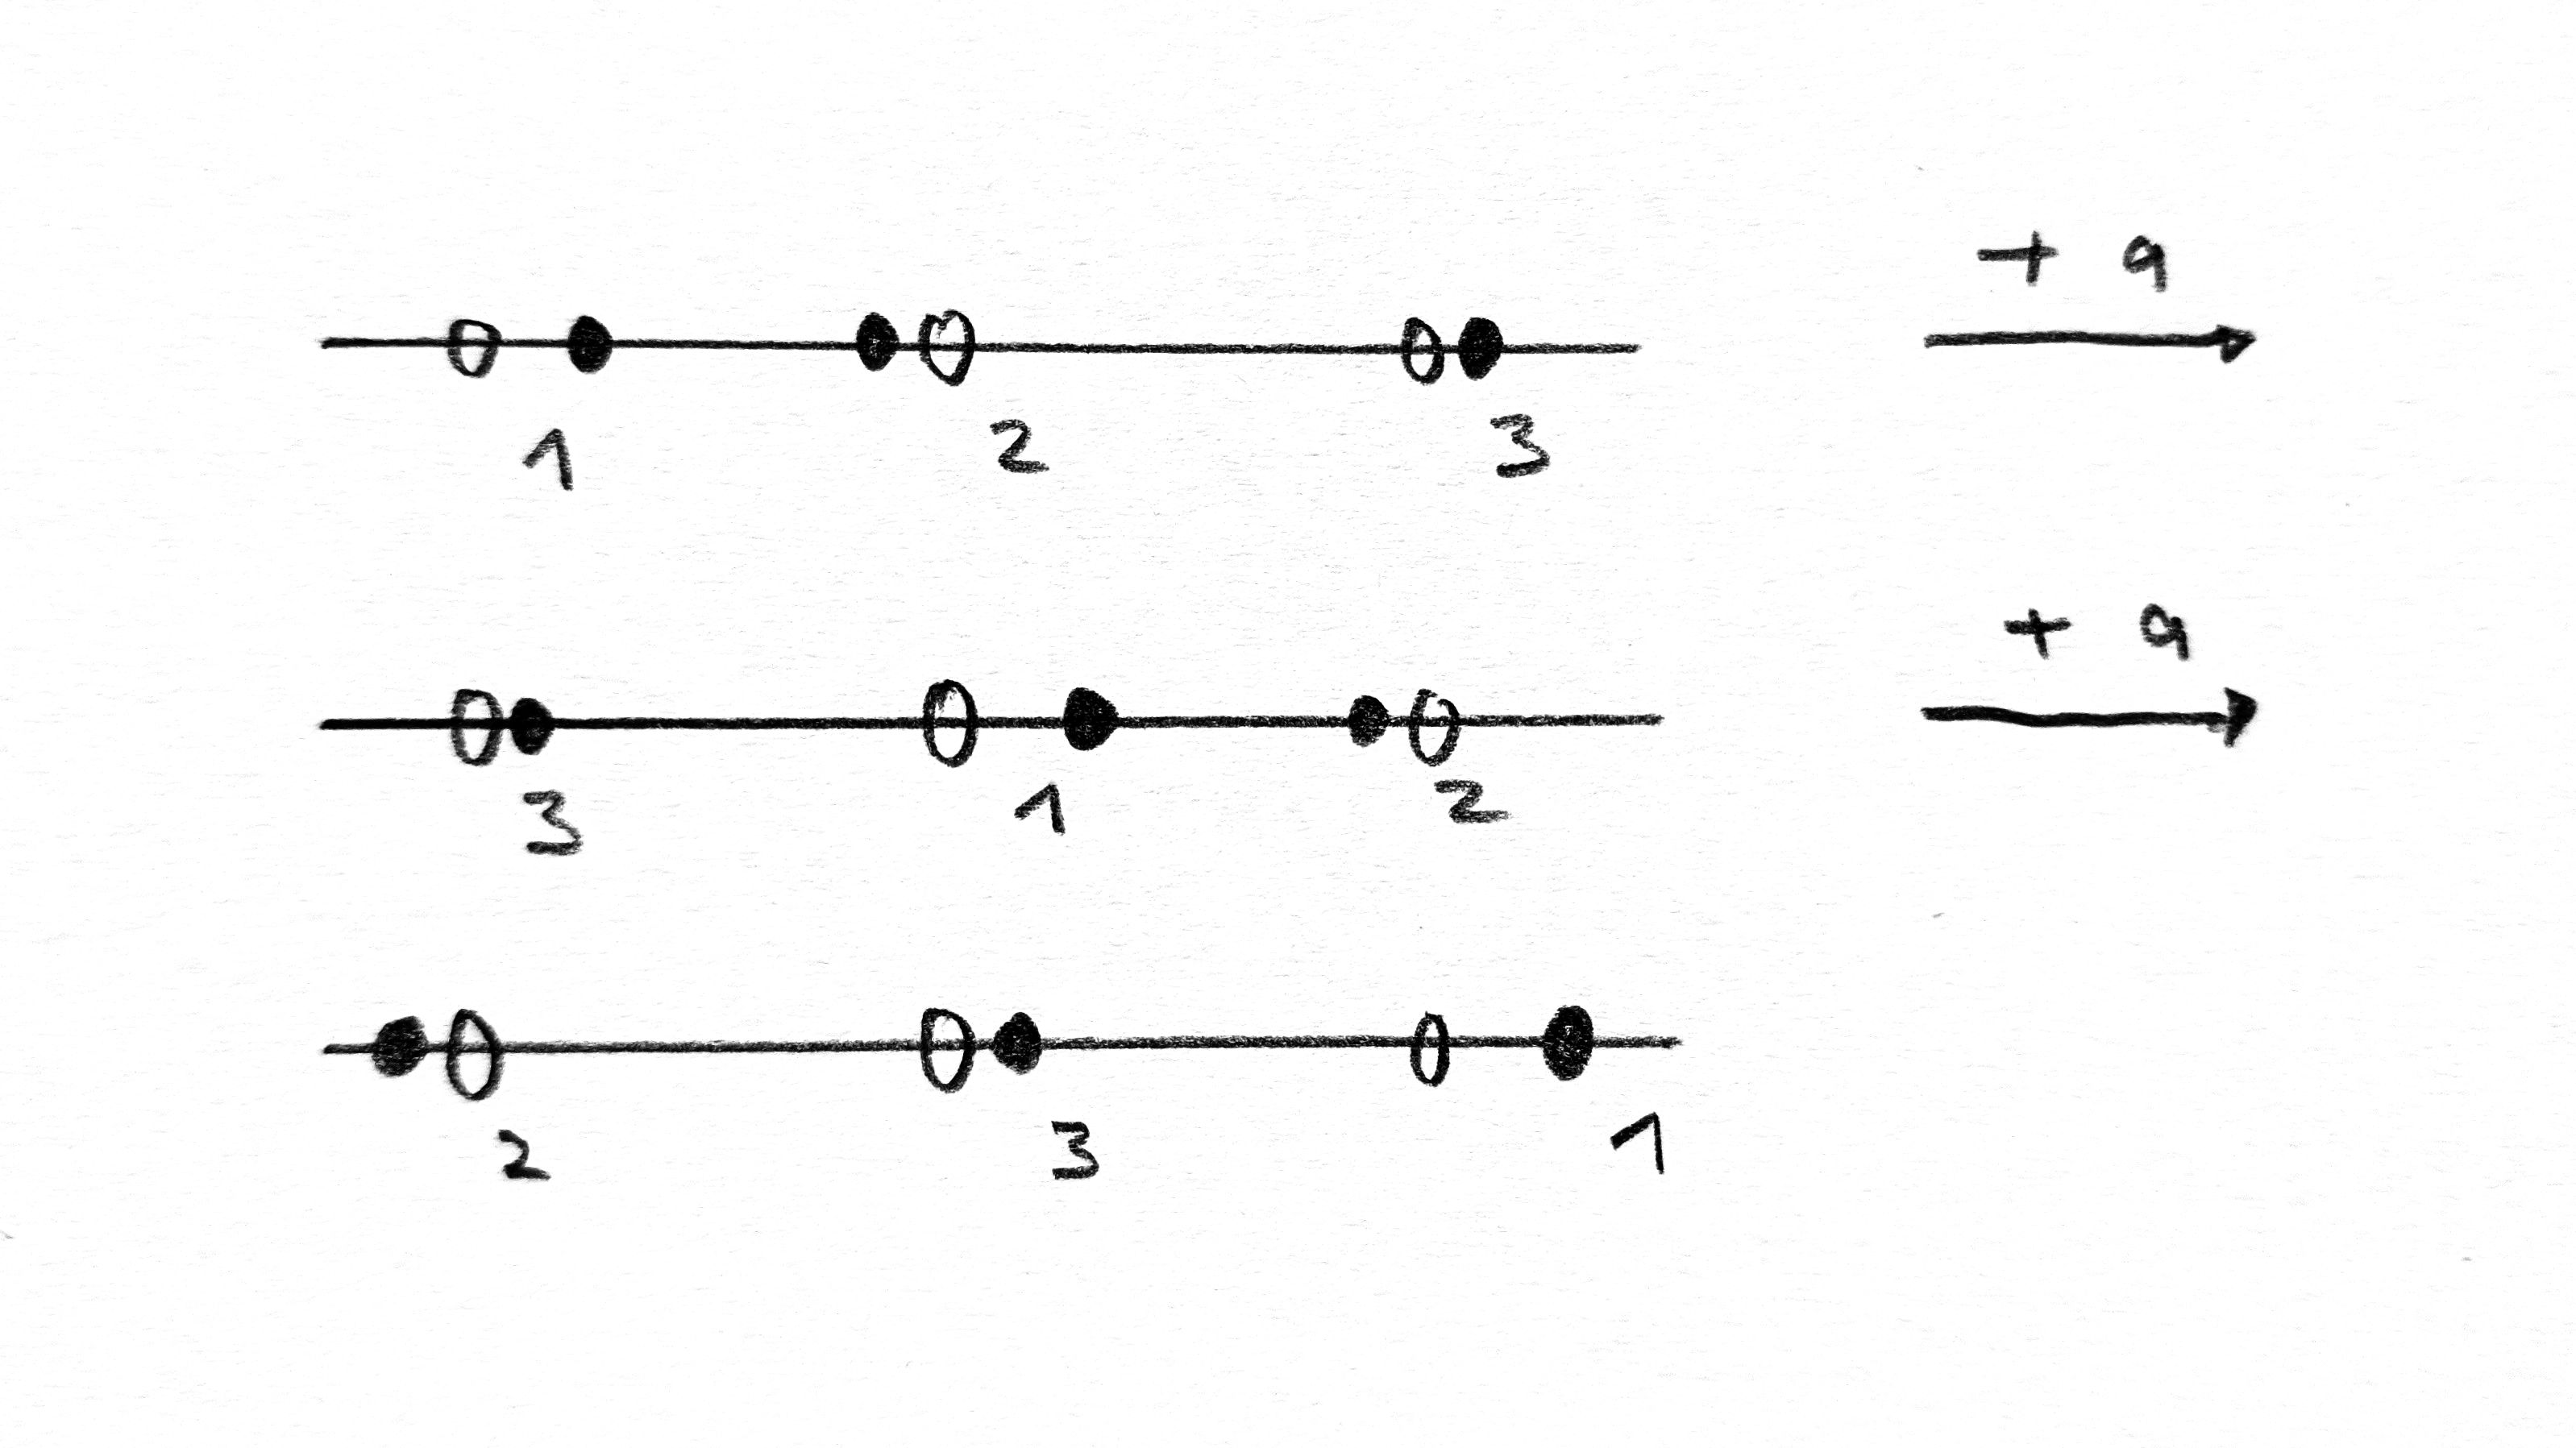
\includegraphics[width=.68\textwidth]{./sketches/permutation1.jpg}
	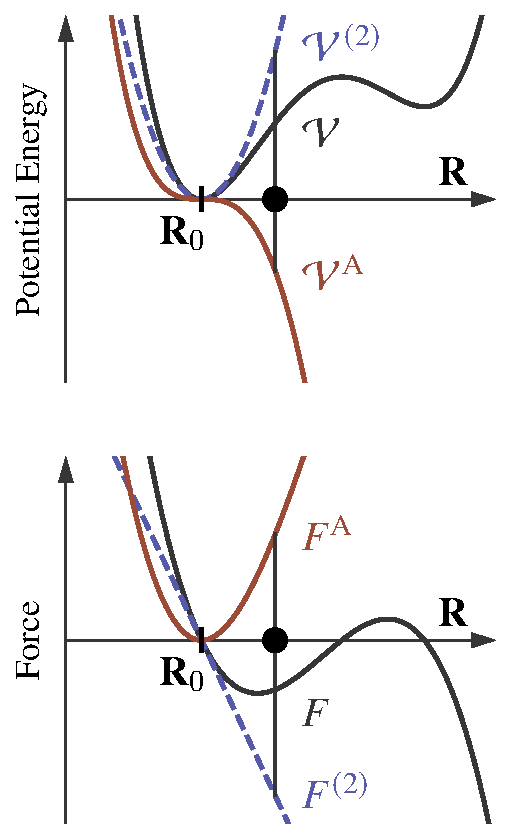
\includegraphics[width=\textwidth]{./data/plots/anharmonicity/1_pes_sketch/sketch_vertical.pdf}
	\caption{Upper: Sketch of a one-dimensional potential-energy surface $\mathcal V$ (solid black), its harmonic approximation $\mathcal{V}^{(2)} (\b R)$ (dashed blue), and the anharmonic contribution $\mathcal{V}^{\rm A} (\b R)$ (solid red). Lower: The force ${F} ({\bf R})$ given by the derivative of $\mathcal V$ (black), the force $F^{(2)}$ stemming from $\mathcal{V}^{(2)} (\b R)$ (blue), and the anharmonic contribution $F^\mathrm{A} = F - F^{(2)}$ (red), cf.~Eq.\,\eqref{eq:anh.F}.}
	\label{fig:pes_sketch_vertical}
\end{marginfigure}


\section{Anharmonicity measure}
\label{sec:anharmonicity_measure}

We base the definition of a measure for anharmonicity on the forces, for two reasons: First, because the forces give microscopic insight, as they can be resolved per atom. Second, the forces are statistically easier to describe, since per configuration $\bf R$, there are $3N$ force components ${\bf F} = ({\bf F}_1, \ldots, {\bf F}_N)$.

In terms of the force contributions defined in Eq.\,\eqref{eq:anh.F}, we define a \emph{measure of anharmonicity}, $\sigmaA$, in the following way:
\begin{align}
	\sigmaA (T)
		% = \frac{\sigma [F^{\rm A}]_T}{\sigma [F]_T}
		= \sqrt{\frac{\sum_{I, \alpha} \braket{(F^{\rm A}_{I, \alpha})^2}_T}{\sum_{I, \alpha} \braket{(F_{I, \alpha})^2}_T}}~,
	\label{eq:sigmaA}
\end{align}
where $F_{I, \alpha}^{(A)}$ is the $\alpha$ component of the (anharmonic) force on atom $I$ and $\braket{\cdot}_T$ denotes a thermodynamic average at temperature $T$. The measure $\sigmaA$ quantifies the anharmonic strength in terms of the standard deviation of the distribution of anharmonic force components at a given temperature, $\sigma [F^{\rm A}]_T$, normalized by the standard deviation of the actual force distribution, $\sigma [F]_T$, The standard deviation of a force distribution is defined as
\begin{align}
	\sigma [F]_T 
		= \sqrt{\frac{1}{3N} \sum_{I, \alpha} \braket{F_{I, \alpha}^2}_T}~.
\end{align}
The effect of normalizing the distribution of forces is shown in Fig.\,\ref{fig:anh.normalization} for the two exemplary materials already discussed in the context of phonon dispersions in Sec.\,\ref{sec:ha.dispersions}, silicon, and the orthorombic perovskite KCaF$_3$. Only after normalizing the forces, a meaningful comparison between materials or across temperatures can be achieved.
\begin{marginfigure}
	\centering
	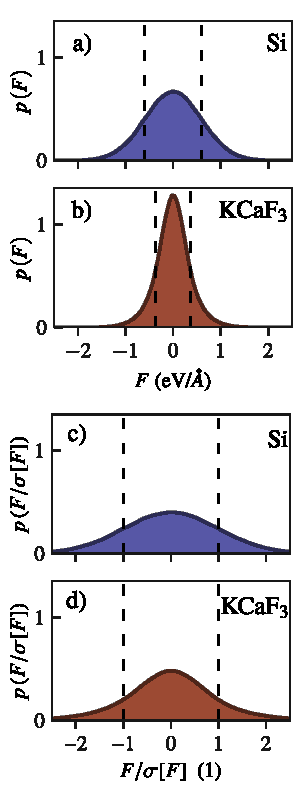
\includegraphics[width=0.8\textwidth]{./data/plots/anharmonicity/4_force_distribution/histogram_forces_vertical.pdf}
	\caption{
		Force component distribution before and after normalization with the width of the distribution $\sigma [F]$. $p(F)$ denotes the probability to find a force component $F_{I, \alpha}$ of strength $F$ in the material. Panel a) and b) show the distribution before normalization, c) and d) after normalization. Dashed vertical lines denotes the standard deviation of the displayed distribution.
	}
	\label{fig:anh.normalization}
\end{marginfigure}


\newthought{For the two exemplary materials, we show the joint normalized distributions of force and anharmonic force contributions} in Fig.\,\ref{fig:anh.sigmaA}, where the thermodynamic sampling is performed by \emph{ab initio} molecular dynamics simulations at 300\,K.
\begin{figure}
	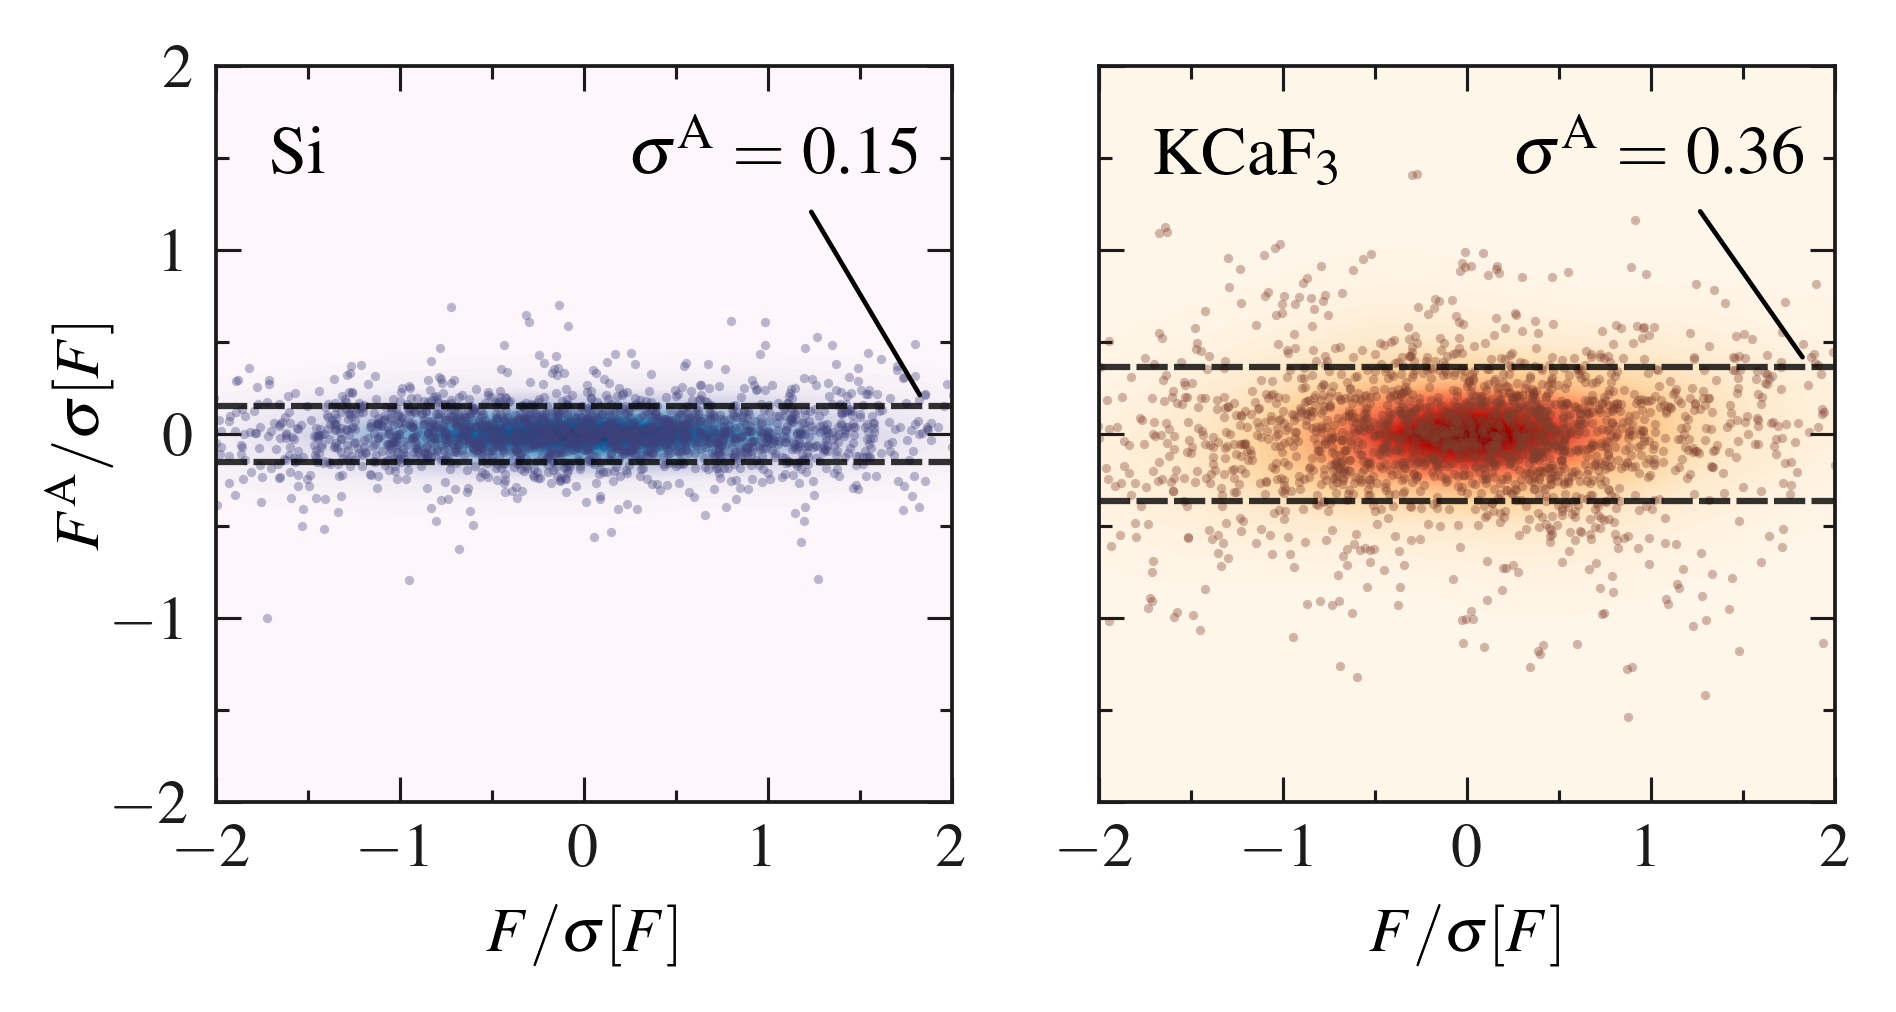
\includegraphics[width=\textwidth]{./data/plots/anharmonicity/5_density_plots/histogram_annotated.png}
	\caption{
		Normalized anharmonic force components versus normalized force components. Dashed horizontal lines: Width of the distribution estimated from standard deviation. Individual dots are force components sampled during an \emph{ab initio} MD simulations.
	}
	\label{fig:anh.sigmaA}
\end{figure}
In this representation, $\sigmaA$ is given by the standard deviation of the distribution in y-direction, as indicated by the dashed horizontal lines in the plot. The distribution of anharmonic force components is more than twice as broad for the perovskite KCaF$_3$ compared to silicon, with a $\sigmaA_{\rm KCaF_3} = 0.36$ compared to $\sigmaA_{\rm Si} = 0.15$. This can be interpreted in the sense that 36\,\% of the forces stem from anharmonic contributions in KCaF$_3$, and 15\,\% in silicon. Furthermore, strongly anharmonic force contributions with a strength of $0.5\,\sigma [F]$ or more are nearly absent in silicon with a probability of $<0.01\,\%$, whereas anharmonic forces of this strength in KCaF$_3$ occur with a much higher probability of $\sim 16.5\,\%$.


\newthought{The anharmonicity measure defined in Eq.\,\eqref{eq:sigmaA}} can also be evaluated for subsets of the dynamical degrees of freedom,~e.\,g.,~per chemical species, as shown in Fig.\,\ref{fig.anh.sigmaA.atoms}.
\begin{figure}
	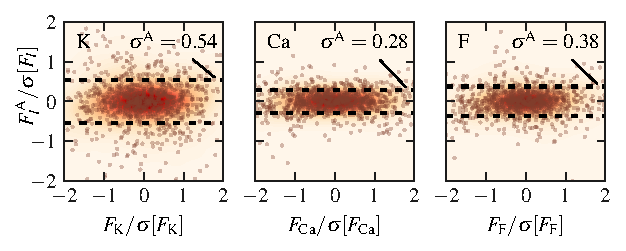
\includegraphics[width=\textwidth]{./data/plots/anharmonicity/5_density_plots/histogram_atoms.pdf}
	\caption{
		Normalized anharmonic force components versus normalized force components. Dashed horizontal lines: Width of the distribution estimated from standard deviation.
	}
	\label{fig.anh.sigmaA.atoms}
\end{figure}
In the example of KCaF$_3$, this analysis shows that the calcium (Ca) atoms occupying the vertices of the unit cell are comparatively well described by the harmonic model, whereas the description of potassium (K) is particularly bad. This can be explained by the phase-transition mechanism observed in KCaF$_3$: Above 560\,K, the material becomes cubic, and the octahedral displacement of fluorine~(F) is removed, as shown in Fig.\,\ref{fig:anh.KCaF3}. This tilt also affects the potassium atoms, which are displaced from their high-temperature reference position in the orthorombic phase, and are therefore located in a shallow potential already at room temperature, well below the phase transition~\cite{Bulou.1980,Hidaka.1984}.
\begin{marginfigure}
	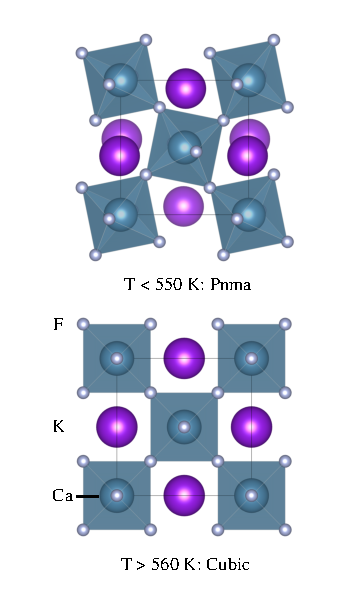
\includegraphics[width=\textwidth]{./data/plots/anharmonicity/2_materials/both.pdf}
	\caption{
		KCaF$_3$ in the low-temperature Pnma~(top) and high-temperature cubic phase~(bottom). Both structures are viewed along the long $b$-axis.
	}
	\label{fig:anh.KCaF3}
\end{marginfigure}

\newthought{It is instructive to evaluate the anharmonicity for single configurations}, be it snapshots in time during molecular dynamics simulations, or when using other sampling approaches,~e.\,g,~harmonic Monte Carlo samples as defined in Eq.\,\eqref{eq:ha.samples}. The sample-resolved anharmonicity is given in analogy to Eq.\,\eqref{eq:sigmaA} as
\begin{align}
	\sigmaA [{\bf R}]
		= \sqrt{\frac{\sum_{I, \alpha} (F^{\rm A}_{I, \alpha})^2}{\sum_{I, \alpha} {(F_{I, \alpha})^2}}}~.
	\label{eq:sigmaA.sample}
\end{align}
While we will discuss ``time-resolved anharmonicity'' in detail at a later point, we show the evaluation of $\sigmaA$ for samples generated by Eq.\,\eqref{eq:ha.samples} in Fig.\,\ref{fig:anh.sampling}.
\begin{figure}
	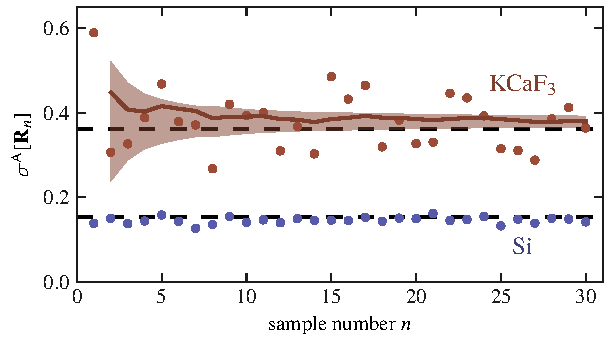
\includegraphics[width=4.1in]{./data/plots/anharmonicity/7_sampling/convergence_sigma_MC.pdf}
	\caption{
			Anharmonicity measure $\sigmaA$ evaluated for individual atomic configurations obtained from Eq.\,\eqref{eq:ha.samples}. Dots: $\sigmaA [{\bf R}_n]$ for individual samples; Red line: Cumulative average.	Black dashed line: $\sigmaA$ from aiMD.	Shadowed region: Convergence estimated by standard error.
	}
	\label{fig:anh.sampling}
\end{figure}
The analysis shows that a decent estimate of $\sigmaA$ can be obtained from the harmonic sampling analysis with few samples. Especially in silicon, each individual harmonic sample yields a $\sigmaA$ within 99\,\% of the reference value obtained by MD simulations for several hundred simulation time steps, which is indicated by the dashed horizontal line. For the more anharmonic KCaF$_3$, the harmonic sampling with 30~samples yields an estimated value of $\sigmaA_{\rm est.} = 0.38$, which differs from the MD value ($\sigmaA = 0.36$) by about 5\,\%. A distinction between largely harmonic materials like silicon, and anharmonic materials like KCaF$_3$, is therefore possible with very few samples.

Motivated by this fact, we investigated the possiblity to estimate $\sigmaA$ based on a single sample, as suggested by Zacharias and Giustino in Ref.\,\cite{Zacharias.2016}: They use a single, deterministic sample to probe the most probable part of the harmonic distribution by choosing $\zeta_s = (-1)^s$ instead of a random distribution in Eq.\,\eqref{eq:ha.samples}. We denote anharmonicity measures obtained by such a ``one-shot'' approach by $\sigmaAOS$ in the following. As shown in Fig.\,\ref{fig:anh.one-shot}, the one-shot samples provide very good estimates for silicon in the the entire temperature range from 200\,K to 800\,K, which can be expected due to the largely harmonic nature of silicon.
\begin{figure}
	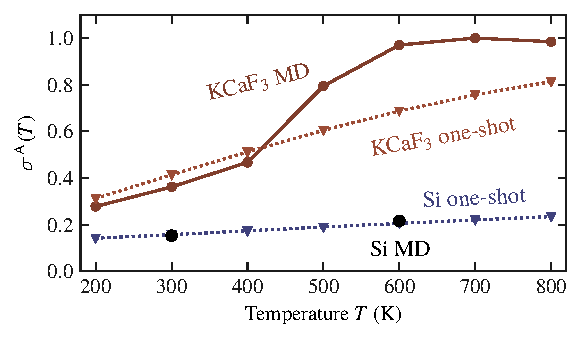
\includegraphics[width=4.1in]{./data/plots/anharmonicity/7_sampling/sigma_temp_one_shot.pdf}
	\caption{
		$\sigmaA$ as a function of temperature obtained from MD~simulations (black circles) and one-shot sampling (triangles connected by dashed curves)
	}
	\label{fig:anh.one-shot}
\end{figure}
For KCaF$_3$, the agreement is decent in the temperature range from 200\, to 400\,K, at least within the limits of the harmonic sampling approach as discussed in the previous paragraph. Above 500\,K, the difference to the reference value from MD simulations increases, which is due to the phase transition mechanism in KCaF$_3$ discussed earlier:
%: This phase transition also occurs in the simulation cell. 
A prediction of anharmonicity across phase transitions cannot be expected from simple harmonic sampling approaches, because the entire reference frame for the harmonic model changes when a phase transition occurs. The phase transition mechanism of KCaF$_3$ and implications for the anharmonicity measure are further discussed in Ref.\,\cite{Knoop.2020}.

\newthought{Ultimately, the applicability of the one-shot sampling approach} needs to be assessed for a diverse set of materials, especially if one aims to use this scheme to screen for anharmonicity in material space. As shown in Fig.\,\ref{fig:anh.screening} for a set of 63~materials, the one-shot sampling is reliable within $\pm 10\,\%$ for all materials in the set, up to a value of about $\sigmaA \simeq 0.2$.
\begin{figure}
	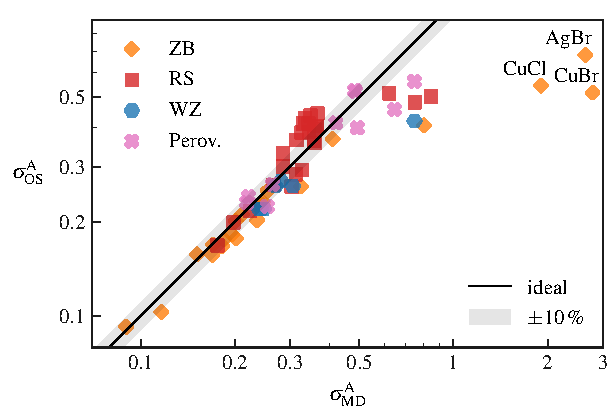
\includegraphics[width=4.1in]{./data/plots/anharmonicity/8_screening/sigma_os_md.pdf}
	\caption{
		Comparison of the anharmonicity measure obtained from MD simulations and one-shot sampling (OS) for 63 materials at 300\,K. The set comprises 25 rock salt (RS), 21 zincblende (ZS), 7 wurtzite (WZ), and 10 orthorombic perovskite (Perov.) materials. The diagonal line denotes perfect agreement between MD and OS, and the green area denotes a 10\,\%~error margin to guide the eye.
		Data was taken from Ref.\,\cite{Knoop.2020}.
	}
	\label{fig:anh.screening}
\end{figure}
For larger values of $\sigmaA$, the deviation can become larger, especially for the group of rock salt materials with $\sigmaA \simeq 0.35$ (red squares) where the one-shot sampling overestimates $\sigmaA$ by about 20\,\%. Nevertheless, the agreement is qualitatively correct up to values of about $\sigmaA \simeq 0.4$, after which materials begin to show effects not captured by the harmonic sampling,~e.\,g.,~phase transitions as discussed earlier for KCaF$_3$. In particular, the three highlighted noble metal halides AgBr, CuCl, and CuBr deviate strongly. These materials tend towards non-perturbative effects during the MD simulation such as spontaneous defect formation~\cite{Knoop.2020}, which is a dynamical effect impossible to describe by any fixed-reference harmonic model. We will discuss the nature of these effects in more detail later in Sec.\,\ref{sec:dynamical_effects}. 

To conclude, we point out that also in the case of non-trivial dynamical effects such as defect formation, the estimated anharmonicity scores $\sigmaAOS$ are larger than $\gtrapprox 0.5$, and therefore indicate strong anharmonicity. A qualitative classification of strong anharmonicity in terms of one-shot sampling is therefore possible for all materials in the set, while quantitative agreement is only achieved for clearly harmonic materials with $\sigmaA \lesssim 0.2$.


\section{Anharmonicity and thermal conductivity}
\label{sec:kappa_vs_sigmaA}

Based on the qualitative discussion of thermal transport in Sec.\,\ref{sec:hf.kappa.ha}, one may expect that stronger anharmonicity leads to shorter phonon lifetimes and therefore lower thermal conductivity. We tested this hypothesis for 47 materials where experimental data was available~\cite{morelLi.2006,Chen.2019}. The results are shown in Fig.\,\ref{fig:anh.kappa}.
%
\begin{figure}
	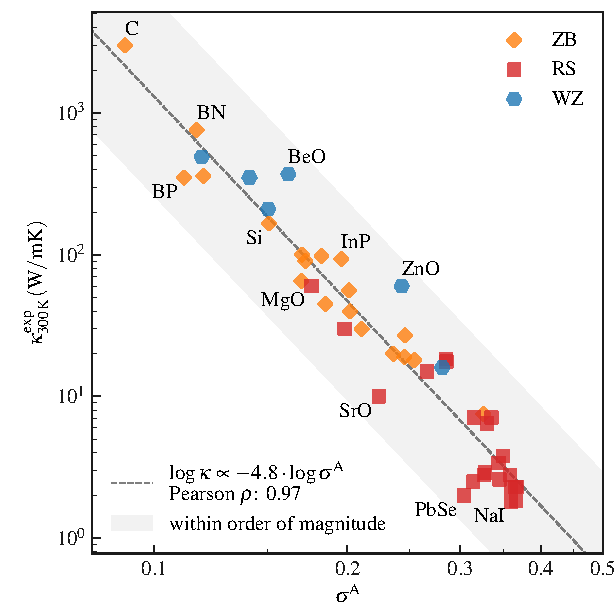
\includegraphics[width=4.1in]{./data/plots/anharmonicity/9_kappa/sigma_vs_kappa.pdf}
	\caption{
		Experimental thermal conductivity at room temperature, $\kappa^{\rm exp}_{300\,{\rm K}}$, versus one-shot measure of anharmonicity, $\sigmaAOS$, and fully anharmonic $\sigmaAMD$ for materials with $\sigmaAOS > 0.2$. 
		The dashed diagonal line indicates a power law fit for the data. The grey area denotes values of $\kappa$ which agree with the fit within 50\,\% to guide the eye. The dataset contains 47 materials, 22 rock salt (RS), 19 zincblende (ZB), and 6 wurtzite (WZ) structures. Experimental data from Ref.~\cite{morelLi.2006,Chen.2019}.
	}
	\label{fig:anh.kappa}
\end{figure}

The analysis reveals an inverse power law relationship between thermal conductivity and anharmonicity for the materials in the dataset,~i.\,e.,~a linear relationship between the logarithms of $\kappa$ and $\sigmaA$, with a Pearson correlation coefficient of 0.97~\cite{Parzen.1960}:
%
\begin{align}
  \kappa (\sigmaA)
    \approx 0.02 \cdot (\sigmaA)^{-4.8}
\end{align}
%
 Given that just a single descriptor is used,~i.\,e.,~the estimated anharmonicity score, and no further vibrational properties as commonly employed in semi-empirical models for thermal condcutivity~\cite{Toberer.2011,Chen.2019}, this correlation is surprisingly good and indicates that $\sigmaA$ captures some essential physics relevant to heat transport: It is known that diamond (C) is extremely harmonic, so that its thermal conductivity is exceptionally high~\cite{Haas.1938,Klemens.1958}. This is confirmed here with diamond being the most harmonic material studied, with $\sigmaA_{\rm C} = 0.09$ and $\kappa_{\rm C} = 3000$\,W/mK~\cite{morelLi.2006}. On average, the zinc blende (ZB) compounds are more harmonic then the rocksalt (RS) compounds in this dataset, and likewise show higher thermal conductivities. This relation can be explained by the stronger covalent bonding character and higher coordination number in the tetrahedrally coordinated zinc blende compounds, compared to the more ionic, octahedrally coordinated rocksalt materials~\cite{Miller.2017}, which explains the clustering of rocksalt materials in the lower right part of Fig.\,\ref{fig:anh.kappa}.
 
 A notable exception in the class of rocksalt materials is the largely harmonic magnesium oxide (MgO), with $\sigmaA_{\rm MgO} = 0.18$ and $\kappa_{\rm MgO} = 60$\,W/mK~\cite{morelLi.2006}.

%\mscomment{Why are the rock salts bottom right?}
%\FK{More ionic character and therefore weaker bonding on average compared to ZB and WZ.}
%\mscomment{tell that these are ``close to harmonic materials''}
%\FK{not sure they are}
%\mscorrect{why Pearson rho? What does it tell?}
%\mscorrect{why is an order of magnitude ok here?}
%\mscorrect{it looks more than an order of magnitude}


\newthought{The most important messages from Fig.\,\ref{fig:anh.kappa} can be summarized as follows}, adopting the definition suggested by Morelli and Slack to define ``high thermal conductivity'' as $\kappa \gtrsim 50 \, {\rm W/mK}$~\cite{morelLi.2006}:
\begin{enumerate}
	\item Very harmonic materials with $\sigmaA \simeq 0.1$, like diamond ($\sigmaA_{\rm C} = 0.09$), boron phosphide ($\sigmaA_{\rm BP} = 0.11$), or boron nitride ($\sigmaA_{\rm BN} = 0.12$) can be expected to be very good thermal conductors with $\kappa \gtrsim 100\,{\rm W/mK}$.
	\item Strongly anharmonic materials with $\sigmaA \gtrsim 0.3$ can be expected to be poor thermal conductors with $\kappa \lesssim 10\,{\rm W/mK}$.
%    \mscomment{would you say 0.3 still works with BTE?}
%    \FK{yes, with more sophisticated approaches than 0K third order, see discussion in \cite{Ravichandran.2018} for NaCl.}
% discussed later
	\item $\sigmaA$ has a strong correlation with thermal conductivity across the entire dataset, but nevertheless only a rough estimate can be made solely based on $\sigmaA$, especially in the middle region with $\sigmaA \simeq 0.2$. This can be seen by comparing strontium oxide (SrO) with $\kappa = 10\,{\rm W/mK}$ and $\sigmaA = 0.22$, and zinc oxide (ZnO) with $\kappa = 60\,{\rm W/mK}$ and $\sigmaA = 0.24$, or beryllium oxide (BeO) with $\kappa = 370\,{\rm W/mK}$ and $\sigmaA = 0.16$ to magnesium oxide (MgO) with $\kappa = 60\,{\rm W/mK}$ and $\sigmaA = 0.18$. These pairs of materials differ only slightly in their estimated anharmonicity, but still quite strongly in the thermal conductivity, clear evidence for the fact that other material properties determine thermal transport. 
% Nevertheless, the correct order of magnitude of $\kappa$ as indicated by the grey area in Fig.\,\ref{fig:anh.kappa} can always be predicted for the investigated materials.
\end{enumerate}

{These findings suggest the following approach} towards screening material space in search for thermal insulators with $\kappa < 10\,{\rm W/mK}$: Estimate the anharmonicity for materials of interest and focus on the anharmonic ones with $\sigmaA > 0.2$, as more harmonic materials will very likely have higher thermal conductivies.
%\mscomment{sounds bad. Are there examples for thermal insulators with $\sigmaA < 02$}
%\FK{not in our data.}
%\ADD{worst example}
%\mscomment{more importantly: can we use BTE yes/no? important for material space exploration}

Of course, the reverse approach could be pursued when searching for materials with potentially high thermal conductivity.

\section{Candidate Materials}
\begin{marginfigure}
	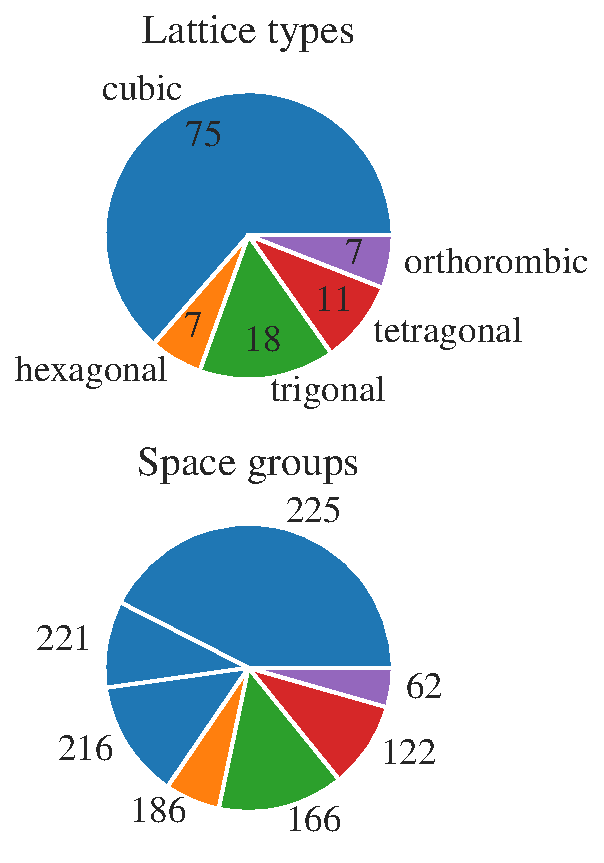
\includegraphics[width=\textwidth]{./data/plots/dataset/pies.pdf}
	\caption{
		Lattice types and space groups represented in the dataset. Space groups not shown in the pie chart: 56, 61, 160, 164, 206, with one representative each.
	}
	\label{fig:anh.pie}
\end{marginfigure}
Using the measure $\sigmaA$, we have identified a set of 118 binary and ternary materials for further investigation.  % with the \emph{ab initio} Green Kubo (aiGK) approach. 
The materials comprise five lattice types and 12 space groups as summarized in Fig.\,\ref{fig:anh.pie}.
%\begin{figure}
%	\includegraphics[width=\textwidth]{./data/plots/dataset/pies_horizontal.pdf}
%	\caption{
%		Lattice types and space groups represented in the dataset. Space groups not shown in the pie chart: 56, 61, 160, 164, 206, with one representative material each.
%	}
%	\label{fig:anh.pie}
%\end{figure}
Since we are mainly interested in thermal insulators as candidate thermoelectric and thermal barrier coating materials, we focus on anharmonic strengths $\sigmaA > 0.2$ as explained above, with a mean of $\sigmaA=0.31$ and a median of $\sigmaA = 0.29$. Some more harmonic materials like MgO ($\sigmaA = 0.18$) have been included for benchmark purposes. A histogram displaying the distribution of $\sigmaA$ values is shown in Fig.\,\ref{fig:anh.histogram}.
\begin{figure}
	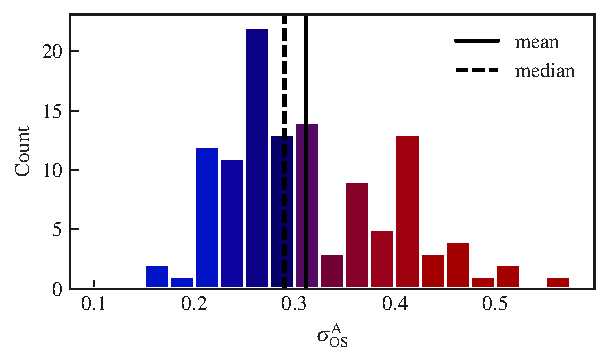
\includegraphics[width=4.1in]{./data/plots/dataset/histogram.pdf}
	\caption{
		Histogram of $\sigmaAOS$ values samples for the 118 chosen materials
	}
	\label{fig:anh.histogram}
\end{figure}
All values are given with respect to room temperature, as this is the regime where the most experimental reference is available to benchmark the aiGK method later on. In total, there are experimental reference values for 45 materials available. The references are given in Tab.\,\ref{tab:kappa.exp} in appendix~\ref{sec:app.experiments}.

\TODO{Include full list of materials with reference in appendix}

The materials have been chosen based on the following criteria:
\begin{enumerate}
	\item Material has to have an experimentally known stable phase at room temperature,
	\item material has to be semiconductor or insulator with a bandgap large enough to prevent accidental gap closing during molecular dynamics simulations,
	% \mscorrect{it was not explained what happens in this case}
	\item the most heavy element considered is Barium ($Z=56$), after which relativistic effects beyond the ``zeroth order regular approximation'' cannot be neglected~\cite{Vanlenthe.1994,Huhn.2017,Zhao.2021}.
    % \mscorrect{ZORA is not explained anywhere}
\end{enumerate}

%\mscorrect{not just application driven, also Q whether BTE works and when it doesn't there is interesting physics}


%\REM{
%The materials come from these sources:
%From Ramprasad: 41
%From Toberer: 3
%From Springer: 4
%From Roekeghem: 9
%From ICSD: 55
%From Seko: 2
%From AAPL: 4
%}



\newpage
\section{Dynamical effects}
\label{sec:dynamical_effects}
As briefly discussed in Sec.\,\ref{sec:anharmonicity_measure},
%shown in the initial screening of material space presented in Ref.\,\cite{Knoop.2020},
%\mscorrect{this is also part of the thesis, don't just cite}
 strongly anharmonic materials with $\sigmaA > 0.3$ are prone to exhibiting non-trivial dynamical effects such as metastable defect formation and precursors of structural phase transitions. 

\newthought{We carried out \emph{ab initio} molecular dynamics simulations}~\footnote{Computational settings: PBEsol function and \emph{light default} basissets. Time step 4-5\,fs such that the fastest motion corresponding to the highest harmonic vibrational frequency is sufficiently sampled, total simulation time at least 30\,ps. Lattice expansion accounted for by minimizing the pressure in the simulation cell according to the scheme outlined in Sec.\,\ref{sec:app.lattice_expansion}. Full details given in appendix \ref{sec:app.computational_details}.} for each of the candidate materials introduced in the previous chapter to see whether the materials exhibit such non-trivial dynamical effects. 
These dynamical effects can be detected by using a time-resolved anharmonicity measure as defined in Eq.\,\eqref{eq:sigmaA.sample},~i.\,e.,~by evaluating the anharmonicity measure for each sample during the MD with $\sigmaA(t) = \sigmaA [{\bf R} (t)]$, and evaluating fluctuations of $\sigmaA (t)$ in terms of its standard deviation ${\rm std} [ \sigmaA ]$ evaluated along a given trajectory. A comparison of $\sigmaA$ values obtained by one-shot sampling, $\sigmaAOS$, and molecular dynamics, $\sigmaAMD$, is shown in Fig.\,\ref{fig:sigma_os_md_dataset}. Materials with a standard deviation larger than ${\rm std} [ \sigmaAMD ] > 0.01$ are highlighted and labeled.
\begin{figure}
	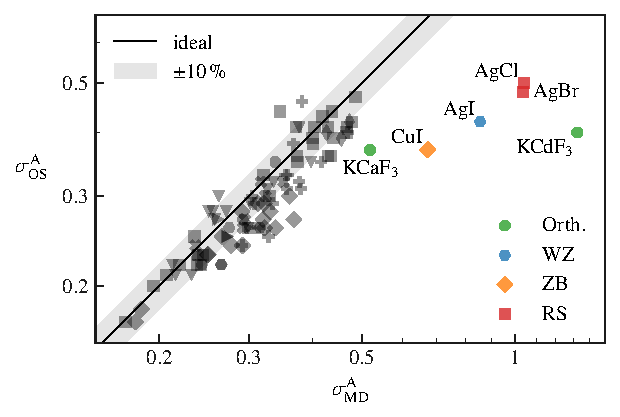
\includegraphics[width=4.1in]{./data/plots/sigma_vs_sigma/sigma_os_md.pdf}
	\caption{$\sigmaA$ values obtained by one-shot sampling (OS) and molecular dynamics simulations (MD) in comparison. Materials with significant fluctuations of the time-resolved anharmonicity measure $\sigmaA (t)$ are highlighted and labeled.}
	\label{fig:sigma_os_md_dataset}
\end{figure}
We discuss the nature of these effects for KCaF$_3$, CuI, AgI, and AgCl in the following. AgBr and KCdF$_3$ are omitted because they behave qualitatively similar to AgCl and KCaF$_3$, respectively. 

The discussion is meant to highlight the prevalence of non-trivial dynamical effects that violate one basic assumption of phonon theory,~i.\,e.,~the assumption of well-defined and stationary reference positions for all atoms in a given phase. Another key insight is that the observed effects are precursors of phase transitions known to occur in these materials at higher temperatures, which means that their onset is observed on the microscopic scale during the dynamic evolution already several 100\,K below the phase transition temperature.
From a methodological point of view, we show how the time-resolved anharmonicity can be used to uncover and explain the nature of the underlying dynamical effect.

%  \mscorrect{honest discussion of simulation times}
%  \FK{this is done for GK, for these static properties 30ps is \emph{grotesquely} overconverged.}
%  \mscorrect{supercell sizes}
%  \FK{beyond the scope of this work, see \cite{Carbogno.2016} for supercell scaling behavior of interpolation scheme}
%  \mscorrect{I would conclude that above $\sigmaA > .2$ non-perturbative calculation should be performed}
%  \FK{I wouldn't.}

\newpage

\subsection{KCaF$_3$}
KCaF$_3$ is the perovskite material already discussed in some detail in Sec.\,\ref{sec:anharmonicity_measure}, where the octahedral tilting mechanism typical for this class of materials, and the phase transition phenomenology were presented~\cite{Bulou.1980,Hidaka.1984,Knight.2005}. In total, we performed five $NVE$ simulations for KCaF$_3$, with a simulation time of 30\,ps each. The time resolved anharmonicity measure is displayed for each of those trajectories in Fig.\,\ref{fig:defects.KCaF3.sigmaA}.
We find that in three of the five trajectories, $\sigmaA (t)$ jumps between the reference value of $\sigmaA \approx 0.4$,\footnote{We round to 1 decimal point in the following, which is completely sufficient for the discussion of intermittent jumps.} and increased values between $\sigmaA \approx 0.8$ and $\sigmaA \approx 1.2$.
%
\begin{figure}
	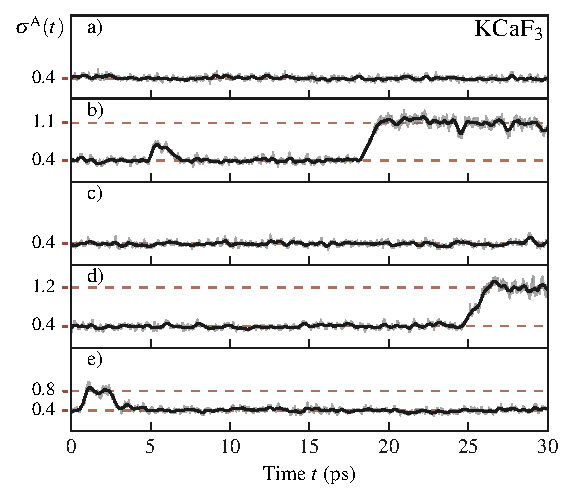
\includegraphics[width=\textwidth]{./data/plots/defects/062.05.KCaF3/sigma_vs_time.pdf}
	\caption{Time-resolved anharmonicity measure $\sigmaA (t)$ for orthorombic KCaF$_3$ in five molecular dynamics runs of 30\,ps length. Increased values of $\sigmaA (t)$ are found in three trajectories (b, d, e).}
	\label{fig:defects.KCaF3.sigmaA}
\end{figure}
%
\newthought{The nature of the underlying dynamical effects} can be resolved by time-averaging the positions ${\bf R} (t)$,
\begin{align}
	{\bf R}_{\rm avg} = \braket{{\bf R} (t)}_t~,	
	\label{eq:R(t).avg}
\end{align}
%
\begin{marginfigure}[-3cm]
	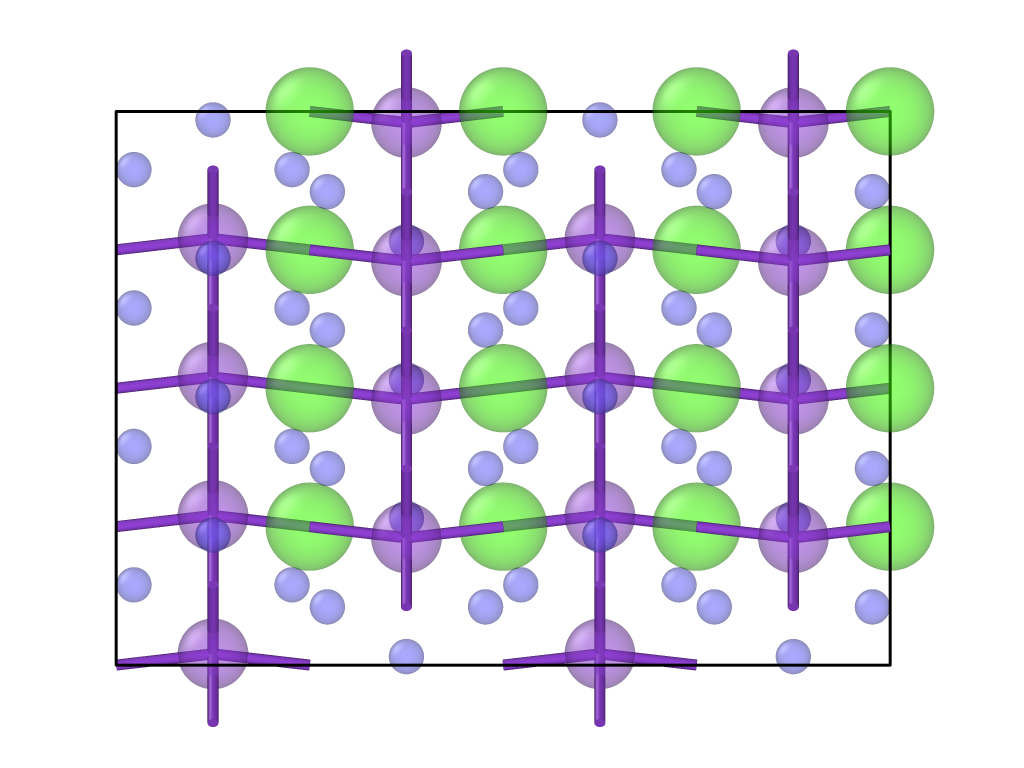
\includegraphics[width=\textwidth]{./data/plots/defects/062.05.KCaF3/plots/ref_left.png}
	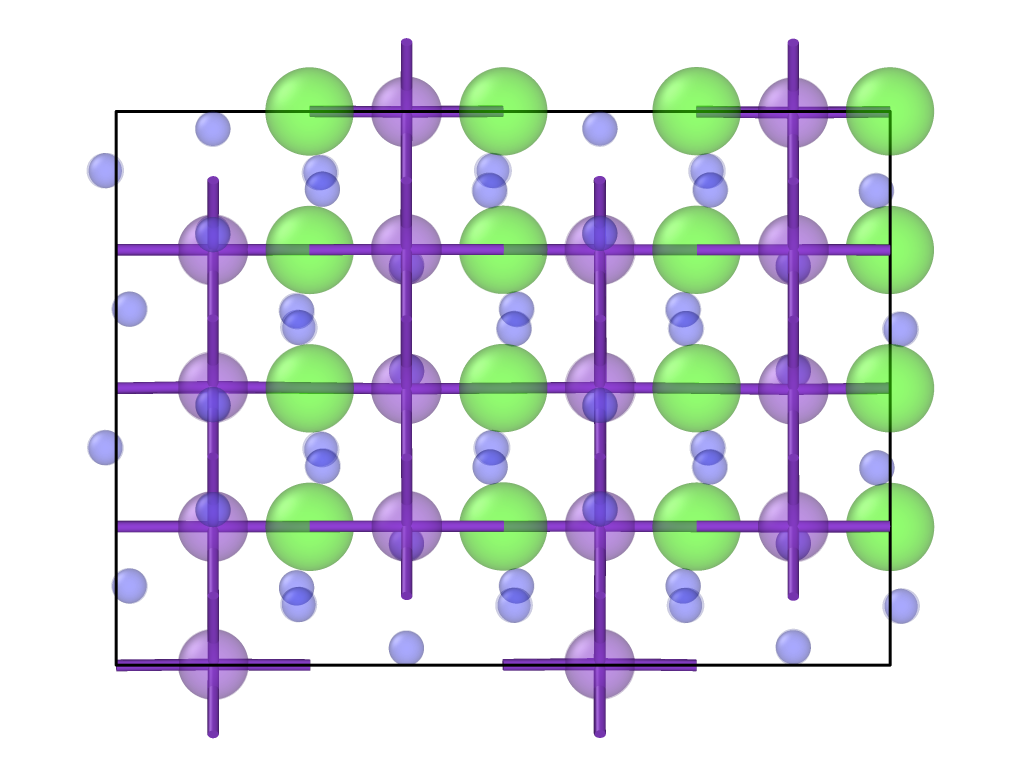
\includegraphics[width=\textwidth]{./data/plots/defects/062.05.KCaF3/plots/2_left.png}
	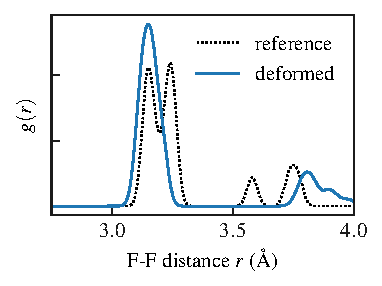
\includegraphics[width=\textwidth]{./data/plots/defects/062.05.KCaF3/rdf/geometry_in_def_2.pdf}
	\caption{Precursor of phase transition in KCaF$_3$. Upper panel: The reference orthorombic structure viewed in (010) direction. The orthorombic displacement of the potassium sub-lattice (violet balls connected by sticks) is clearly visible. Middle panel: When $\sigmaA (t) \approx 1.1$, the potassium sub-lattice temporarily adopts a tetragonal shape. Also the fluorite atoms (small blue balls) reduce their tilt consequently. Lower panel: Radial distribution function $g(r)$ for the fluorine atoms in the orthorombic reference and deformed structure: The number of distinct peaks reduces, reflecting an increase in symmetry when the orthorombic tilt reduces.}
	\label{fig:defects.KCaF3.1}
\end{marginfigure}
\noindent
for the time spans in which $\sigmaA (t)$ is increased. Performing this time average for time spans where $\sigmaA (t) < 0.5$,~i.\,e.,~in situations in which no increase is seen, one recovers the initial orthorombic structure shown in Fig.\,\ref{fig:defects.KCaF3.1} (top figure). When averaging trajectory b) for the time where $\sigmaA (t) \approx 1.1$, the resulting structure is more symmetric, with an approximately tetragonal arrangement of atoms. This can be seen by focusing on the potassium sub lattice (purple atoms connected by sticks) in Fig.\,\ref{fig:defects.KCaF3.1} (middle). The increased symmetry is further revealed by noting that the fluorine cage becomes more ordered, as shown in terms of the F-F pair distribution function in Fig.\,\ref{fig:defects.KCaF3.1} (bottom). This phenomenon can be viewed as a precursor of the phase transitions towards tetragonal and cubic phases known to occur in this material at temperatures higher than 560\,K~\cite{Bulou.1980,Hidaka.1984,Knoop.2020}. However, at 300\,K, well below the transition temperature, this configuration only occurs sporadically on the time scale of several picoseconds during the simulation, and is therefore not fully stabilized.

%\mscorrect{it is not expected that the full supercell adopts the structure but only one/few atoms}
%\FK{Fig. \ref{fig:defects.KCaF3.1} clearly shows that we observe a collective effect and not single atom defects.}

% \newpage

\subsection{CuI}
\label{sec:defects.CuI}

\begin{figure}
	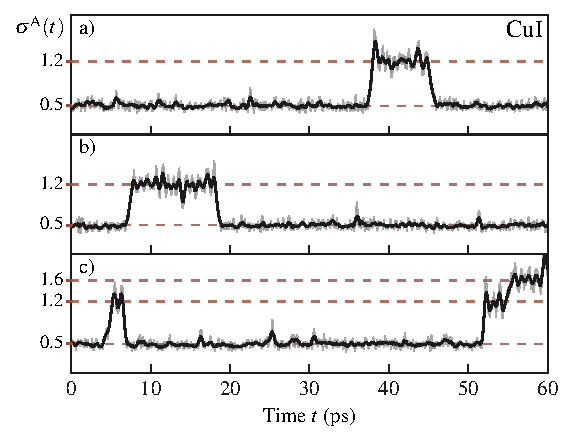
\includegraphics[width=\textwidth]{./data/plots/defects/216.02.CuI/sigma_vs_time.pdf}
	\caption{Time-resolved anharmonicity measure $\sigmaA (t)$ for zincblende CuI in three molecular dynamics runs of 60\,ps length. Increased values of $\sigmaA (t)$ are found in all three trajectories.}
	\label{fig:defects.CuI}
\end{figure}
%
%\mscomment{why don't you show pair distribution function for the time snapshots}
%\FK{I tried by it's difficult to normalize because only 1 of 216 atoms moves. It would be an interesting project to do proper coarse graining on this.}
%
Copper iodide (CuI), also known as marshite, is a simple material with fcc lattice of the zincblende type. This phase is also known as the $\gamma$ phase ($\gamma$-CuI).
The time-resolved anharmonicity measures are shown in Fig.\,\ref{fig:defects.CuI} for three trajectories of 60\,ps simulation time.
The characteristic features are the jumps in $\sigmaA (t)$ from values of $\sigmaA (t) \approx 0.5$ to $\sigmaA (t) \approx 1.2$ or 1.6. In the simulated time period, these values are taken for 3 to 12\,ps, before the initial value of $\sigmaA (t) \approx 0.5$ is restored. 
% The jumps in $\sigmaA (t)$ hint at a dynamical effect which strongly violates the harmonic approximation.
%
\begin{marginfigure}
	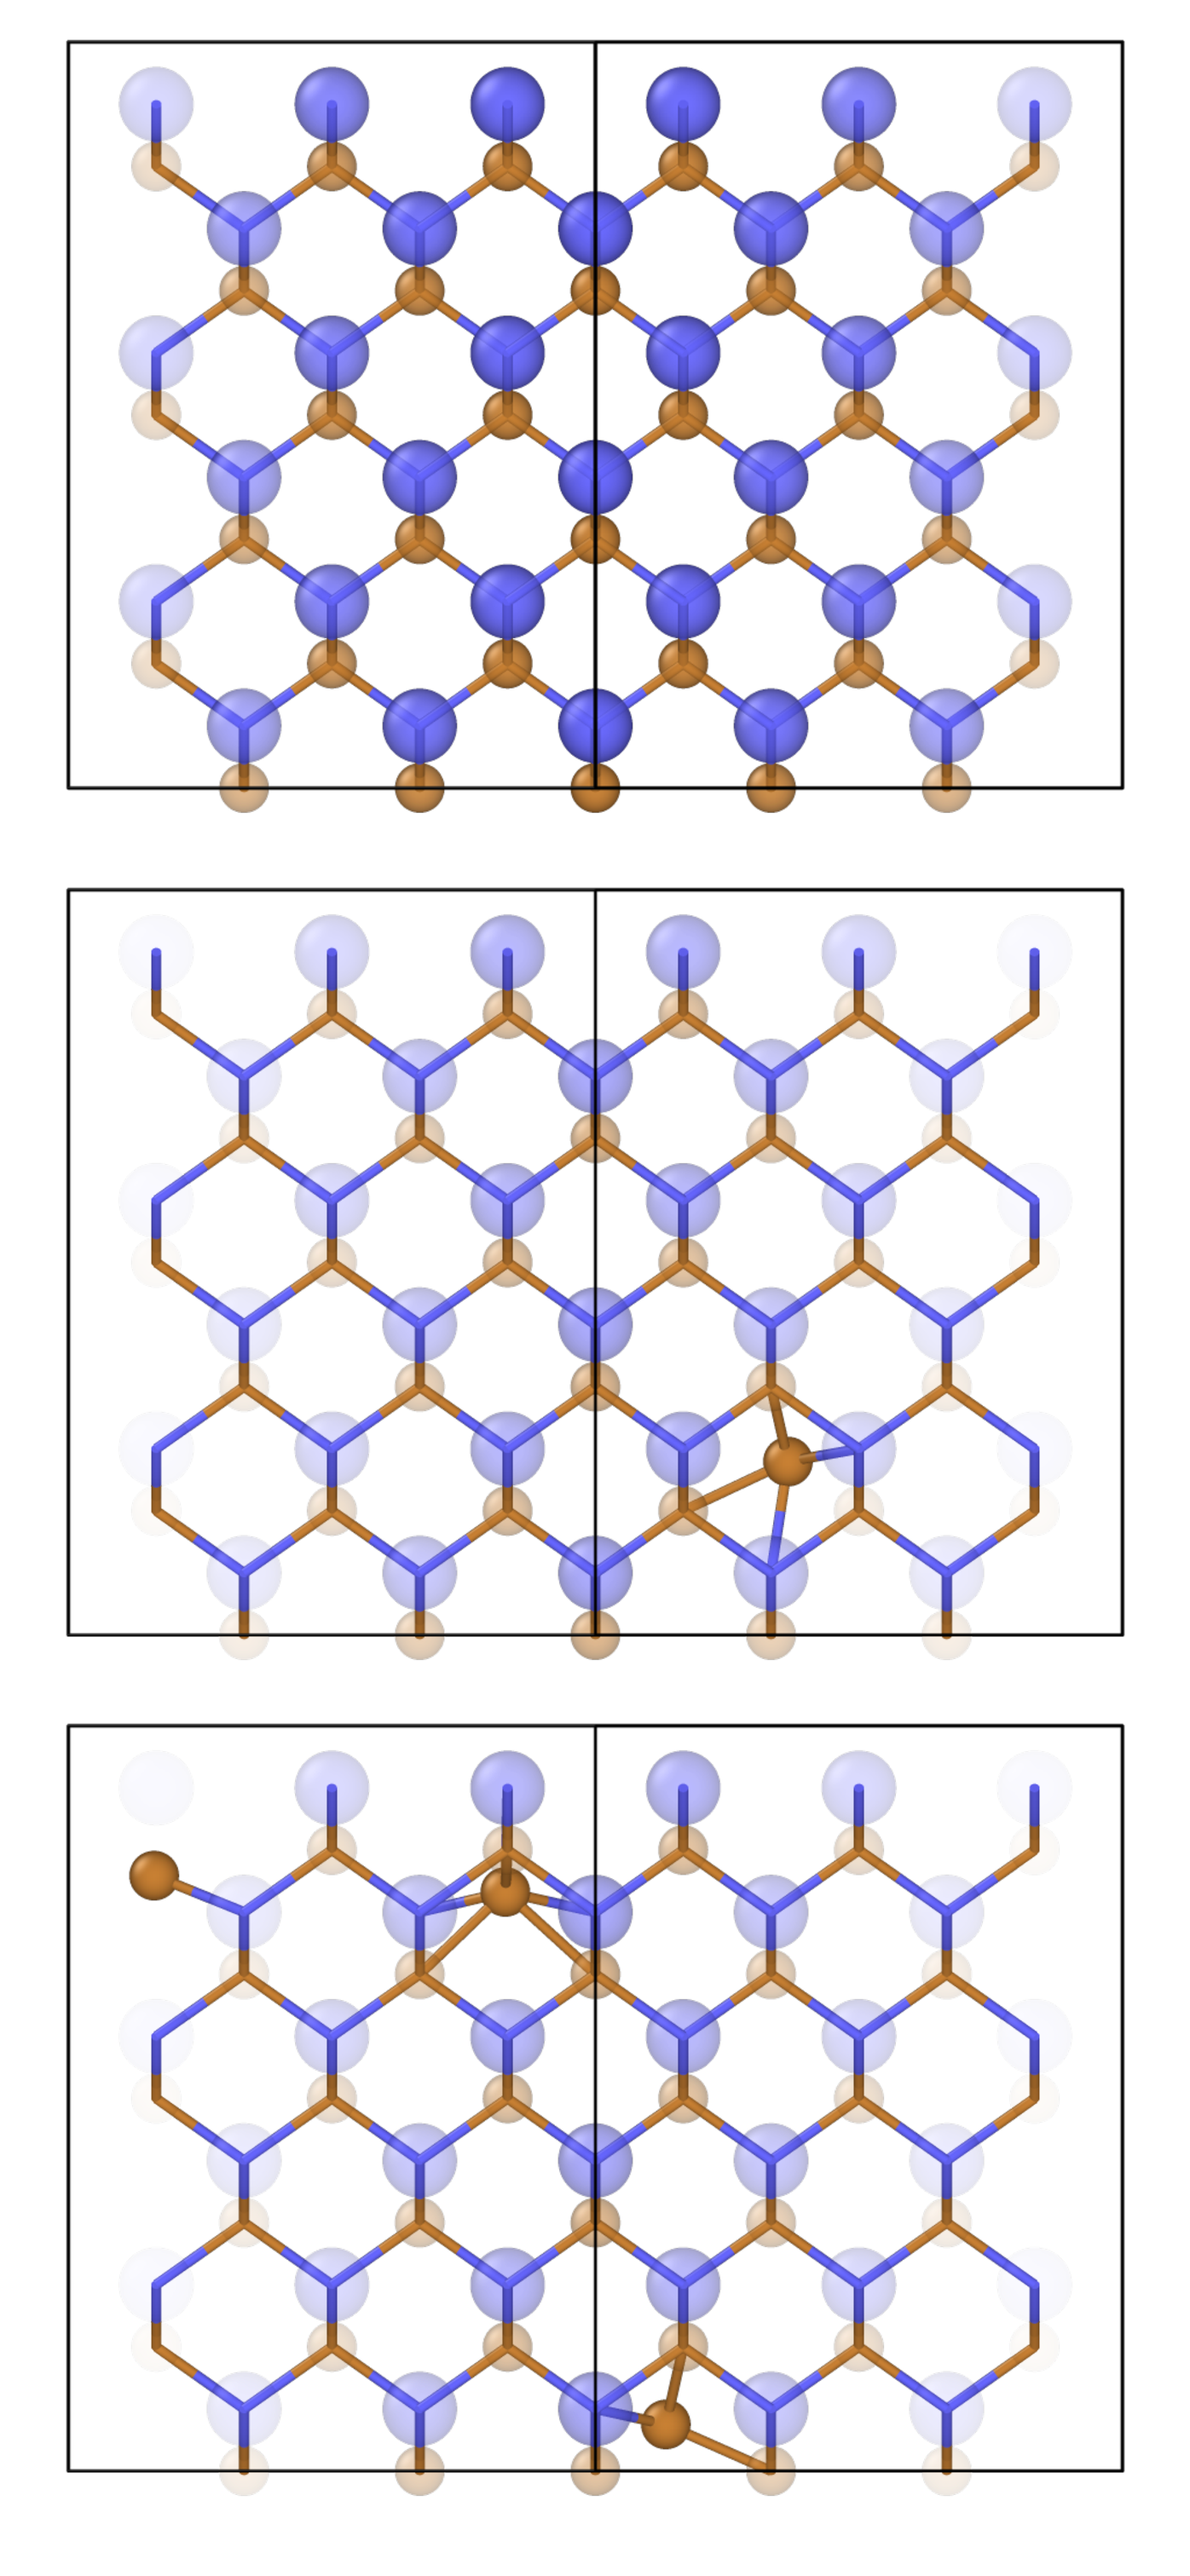
\includegraphics[width=\textwidth]{./data/plots/defects/216.02.CuI/all.pdf}
	\caption{CuI viewed in (110) direction. Top: High-symmetry zincblende structure. Middle: Copper ion in lower-right quadrant moves into interstitial site along (111) direction when $\sigmaA (t) \approx 1.2$. Bottom: Several defects form when $\sigmaA (t) \approx 1.6$}
	\label{fig:defects.CuI.1}
\end{marginfigure} 
%
As in the case of KCaF$_3$, we compare two time-averaged structures in Fig.\,\ref{fig:defects.CuI.1}: A time average with respect to the entire simulation time reveals the perfect zincblende structure of CuI which corresponds to the minimum of the potential-energy surface.
When averaging over the time span where $\sigmaA (t) \approx 1.2$, however, the average structure has one Cu atom diplaced along the (111) direction. Viewing the supercell in (110) direction, the diplacement is clearly visible (Fig.\,\ref{fig:defects.CuI.1}, middle). This means that the Cu occupies a metastable interstitial site at the given position for the respective time period. When $\sigmaA (t)$ is restored to the base value of $\sigmaA (t) \approx 0.5$, the Cu atom moves back to the high-symmetry reference position within the zincblende structure. 
The third trajectory shown in Fig.\,\ref{fig:defects.CuI}~c) evolves to a situation where $\sigmaA \approx 1.6$. This corresponds to a situation, where more than one defects forms~(Fig.\,\ref{fig:defects.CuI.1}, bottom).

\newthought{$\gamma$-CuI is known to undergo a phase transition to a superionic conducting $\beta$ phase} above 643\,K~\cite{Boyce.1979, Boyce.1980,Boyce.1981,Keen.1995}. It is very likely that the defect formation observed in the aiMD simulations at 300\,K are precursors of this phase transition, but too infrequent at this temperature to destabilize the fcc lattice of the $\gamma$ phase.
%\mscorrect{also the other embryos don't destabilize the stable phase}
%\FK{I don't understand, sorry.}

\subsection{AgI}
Wurtzite silver iodide ($\beta$-AgI), or iodargyrite, is another transition metal halide that shares some similarities with $\beta$-CuI discussed in the previous section~\cite{Boyce.1981}. It is known to transition into the superionic conducting $\alpha$ phase above $\sim 420$\,K~\cite{Hoshino.1957,Boyce.1981,Brenner.2020}, and was in fact one of the earliest studied materials exhibiting this phenomenon~\cite{Strock.1934,Strock.1935,Strock.1936}.
%
\begin{figure}
	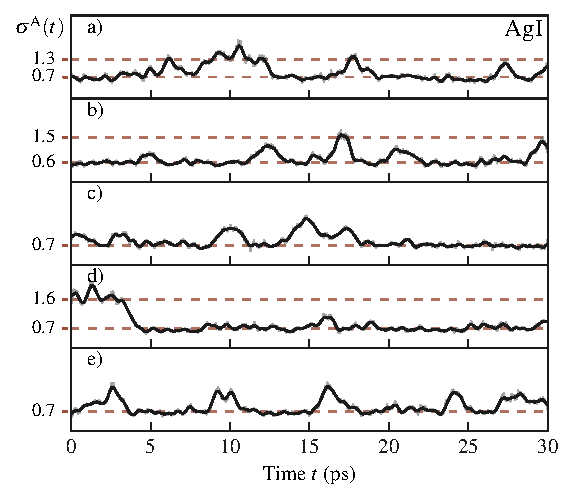
\includegraphics[width=\textwidth]{./data/plots/defects/186.02.AgI/sigma_vs_time.pdf}
	\caption{Time-resolved anharmonicity measure $\sigmaA (t)$ for wurtzite AgI in five molecular dynamics runs of 30\,ps length. Increased values of $\sigmaA (t)$ are found in all five trajectories.}
	\label{fig:defects.AgI}
\end{figure}
%
\begin{marginfigure}
	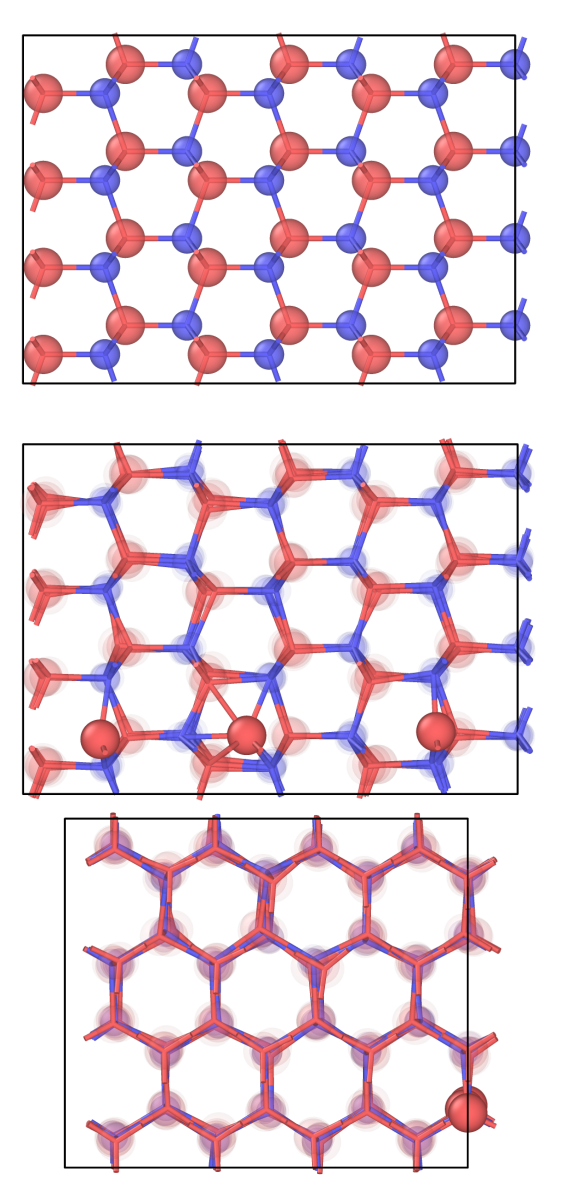
\includegraphics[width=\textwidth]{./data/plots/defects/186.02.AgI/defects_all.png}
	\caption{AgI viewed in (100) direction. Top: High-symmetry wurtzite structure. Middle: Silver ions (red) move into interstitial sites along (001) direction when $\sigmaA (t) \approx 1.3$. Bottom: The same configuration viewed along (001) direction.}
	\label{fig:defects.AgI.1}
\end{marginfigure} 
%
The time-resolved anharmonicity measure for AgI at 300\,K is shown in Fig.\,\ref{fig:defects.AgI}. As in $\gamma$-CuI, the value jumps back and forth between the already quite large reference value of $\sigmaA \approx 0.7$, short spikes at $\sigmaA \approx 0.5$, and longer periods where $\sigmaA \approx 1.3-1.6$ for several picoseconds. For example, the first trajectory displayed in Fig.\,\ref{fig:defects.AgI}~a) jumps between $\sigmaA \approx 0.7$ and $\sigmaA \approx 1.3$ several times, where the longest time span around this value is about 5\,ps. Averaging the positions over this time span as before, we obtain a supercell containing three Ag defects moving along (001) direction in the supercell, as shown in Fig.\,\ref{fig:defects.AgI.1} (middle and bottom), as opposed to the reference wurtzite structure (top).
It is again very likely that the instability of the wurtzite lattice towards defect formation at room temperature is a precursor of the actual phase transition taking place at temperatures approximately 120\,K higher. 

\newpage
\subsection{AgCl}
Silver chloride (AgCl) is yet another material of the class of transition metal halides, and the room-temperature stable phase is rock salt~\cite{Lowndes.1972,Andreoni.1983,Batchelor.1995}.
\begin{figure}
	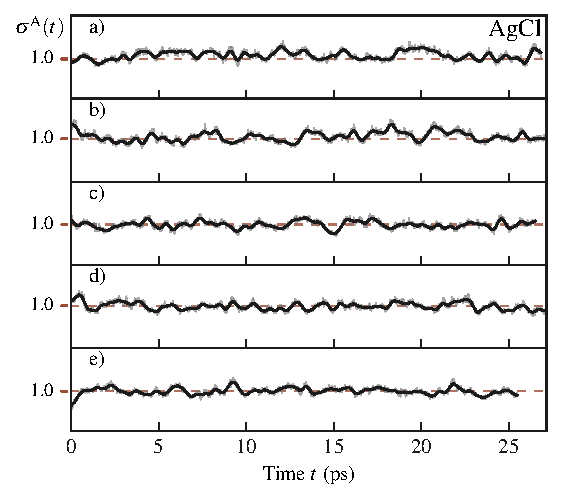
\includegraphics[width=\textwidth]{./data/plots/defects/225.02.AgCl/sigma_vs_time.pdf}
	\caption{Time-resolved anharmonicity measure $\sigmaA (t)$ for rock salt AgCl in five molecular dynamics runs of 30\,ps length. No temporarily increased value of $\sigmaA (t)$ is observed.}
%	\mscomment{pair distribution function?}
%	\FK{see Fig. \ref{fig:defects.pdf.agcl}}
	\label{fig:defects.AgCl}
\end{figure}
%
\begin{marginfigure}[-2in]
	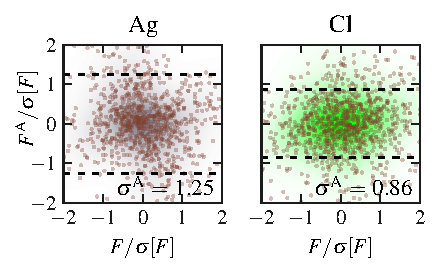
\includegraphics[width=\textwidth]{./data/plots/defects/225.02.AgCl/per_atom/histogram_atoms_margin.pdf}
	\caption{Species-resolved anharmonicity score in AgCl.}
	\label{fig:defects.AgCl.sigmaA}
\end{marginfigure}
%
As opposed to the previously discussed transition metal halides CuI and AgI, the time-resolved anharmonicity $\sigmaA (t)$ exhibits no ``jumps'' in AgCl, but rather stays close to $\sigmaA \approx 1$, which can be interpreted as a situation where the harmonic model loses predictive power for the observed forces.\footnote{$\sigmaA \approx 1$ signals a situation where the anharmonic contribution to the forces becomes as strong as the forces themselves.} By resolving the anharmonicity measure per atom species in Fig.\,\ref{fig:defects.AgCl.sigmaA} similar to the discussion for KCaF$_3$ in Sec.\,\ref{sec:anharmonicity_measure}, we see that the forces on chlorine atoms are better described by the harmonic model with $\sigmaA_{\rm Cl} = 0.86$ than those on silver with $\sigmaA_{\rm Ag} = 1.25$. 
%\mscorrect{performs?}
%\FK{is more predictive?}
This is in line with the previous observations in metal halides where small cations proved to be more mobile and susceptible to dislocations~\cite{Boyce.1979,Brenner.2020}. However, no clear-cut dislocation pattern can be identified for AgCl as opposed to CuI and AgI.
%
\begin{figure}
	\centering
	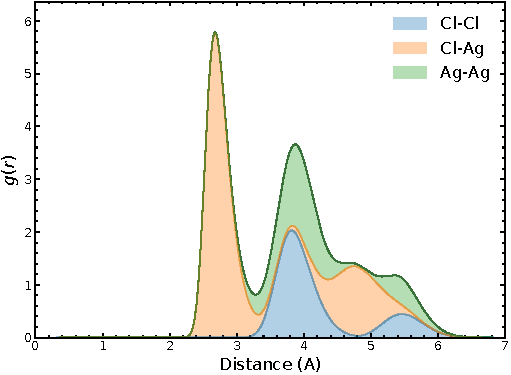
\includegraphics[width=3.5in]{./data/plots/pdfs/agcl.pdf}
	\caption{Pair discribution function for first four coordination shells of rock salt (SG\,225) AgCl.
%	Coordination shells: 
%	1: 2.75579 atoms: Cl-Ag 
%	2: 3.89727 atoms: Ag-Ag/Cl-Cl 
%	3: 4.77317 atoms: Ag-Cl 
%	4: 5.51158 atoms: Ag-Ag	
%	\mscorrect{fix!}
}
	\label{fig:defects.pdf.agcl}
\end{figure}
%
\newthought{The nature of the dynamical effects manifesting in AgCl can nevertheless be elucidated.} We do this by computing the pair distribution functions for the first four coordinates shells in AgCl~\cite{AllenTildesley}, as shown in Fig.\,\ref{fig:defects.pdf.agcl}, and contrasting them with the prototypical, largely harmonic rock salt material magnesium oxide (MgO, $\sigmaA = 0.17$) in Fig.\,\ref{fig:defects.pdf.mgo.small}. 
%
\begin{marginfigure}
	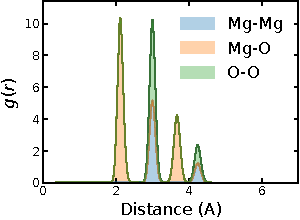
\includegraphics[width=\textwidth]{./data/plots/pdfs/mgo_small.pdf}
	\caption{Radial distribution function resolved by pair contributions.}
	\label{fig:defects.pdf.mgo.small}
\end{marginfigure}
%
In MgO, the distribution of atoms are narrowly distinguishable, which means that the atoms vibrate closely around their reference position, a typical feature of harmonic dynamics. 
%\mscomment{isn't this a sing of harmonic behavior?}
%\FK{Exactly.}
In AgCl on the other hand, only the first coordination shell of silver-chlorine atoms is distinct at 300\,K. The chlorine (Cl-Cl) and silver (Ag-Ag) sublattices (purple/green area in Fig.\,\ref{fig:defects.pdf.agcl}) show discernible peaks, although the broadening is significant compared to MgO. The silver-chlorine (Cl-Ag) distribution (yellow area) is even more broadened and is still non-zero at distances normally characteristic of like atoms (Cl-Cl or Ag-Ag) , see~e.\,g.,~the non-zero width of the yellow curve at 3.9 and 5.5\,\AA (second and fourth coordination shell). In total, this leads to a very strong broadening in the third and fourth coordination shell, with a barely discernible local maximum in the third coordination shell (4.8\,\AA).
This is in line with experimental Extended X-ray Absorption Fine Structure (EXAFS) measurements detecting an ``anomalously large motion'' in the third neighbor shell already at a temperature of 120\,K~\cite{Batchelor.1995}.
This hints at severe dynamical distortions throughout the simulation which are typically discussed in terms of dynamical Frenkel pair formation, where the mobile Ag$^+$ cations dynamically populate interstitial sites~\cite{Aboagye.1975,Andreoni.1983,Wilmer.1995,Mebane.2010}. While we can confirm an increased mobility of Ag$^+$ ions as discussed above, we do not observe a local accumulation of Ag$^+$ ions at interstitial sites, which should correspond to additional local maxima in the respective pair distribution functions compared to the reference structure. 
%
%\mscomment{minima? maxima?}
%\FK{maxima probably correct}
\mscomment{where would interstitial be in Fig. 4.21?}
\FK{check!}
%
However, such an effect might very well occur at higher temperatures, and the observed effects are fingerprints of the instability of the lattice towards this kind of dynamical defect formation.
Irrespective of the exact type of defect formation, %which is beyond the scope of this work, 
the observed dynamical effect hints at a strong form of premelting phenomenon in AgCl, which has an experimental melting temperature of 728\,K.

\newthought{Similar effects can be observed in silver bromide (AgBr)}. As discussed in Ref.\,\cite{Andreoni.1983}, the dynamical properties of AgCl and AgBr share many similarities with the chemically related material AgI presented in the previous section. In contrast to AgI however, they do not become superionic conductors before melting, despite the increased ion mobility presented here.
%\mscomment{this is not your results}
%\FK{true}

\section{Anharmonicity and Boltzmann Transport}
\label{sec:anharmonicity.bte}
As previously mentioned, there are two established approaches to compute thermal conductivities in solids from first principles: Fully anharmonic Green Kubo simulations, and Boltzmann transport theory with perturbative treatment of phonon-phonon interactions. 

In order to assess the need for non-perturbative simulations, 
% even in simple materials, 
we have reproduced thermal conductivities calculated by a state-of-the-art Boltzmann transport approach published by Xia and coworkers in Ref.\,\cite{Xia.2020} in the light of the previously introduced anharmonicity measure $\sigmaA$ in Fig.\,\ref{fig:anh.bte}.
%
\begin{figure}
	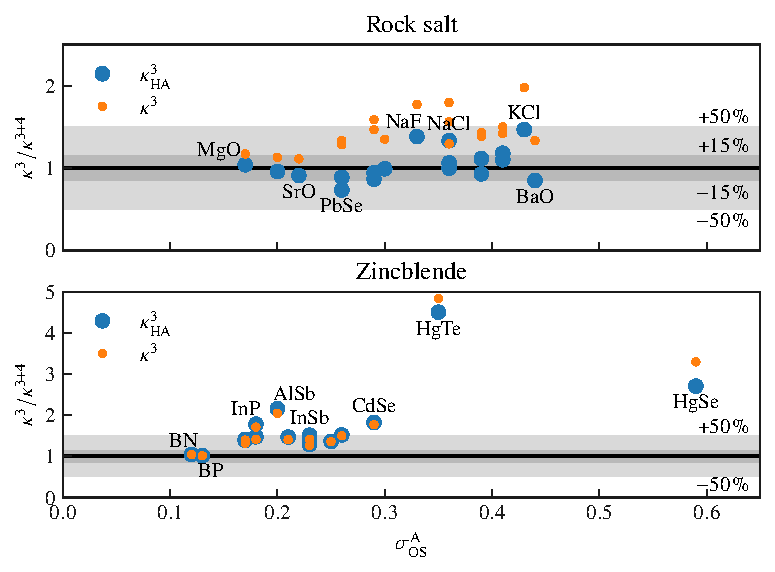
\includegraphics[width=4.1in]{./data/plots/BTE_comparison/k_34.pdf}
	\caption{
		Boltzmann transport calculation of thermal conductivity at room temperature including third- and fourth-order contributions to the potential-energy surface for 34 zinc blende and rocksalt compounds from Ref.\,\cite{Xia.2020}. $\kappa^3_{\rm HA}$: Boltzmann transport with three-phonon scattering rates computed from third-order terms, cf. Eq.\,\eqref{eq:Gamma_s}. $\kappa^3$: Boltzmann transport with three-phonon scattering and additionally accounting for phonon-frequency renormalization via self-consistent phonon theory~\cite{Xia.2018}. These approximations are compared with $\kappa^{3+4}$,~i.\,e.,~the highest available level of theory where both frequency renormalization and four-phonon scattering are additionally included in the computation of thermal conductivity. The data points give the relative change with respect to $\kappa^{3+4}$,~i.\,e.,~1 means perfect agreement between different levels of theory.
	}
	\label{fig:anh.bte}
\end{figure}

The figure shows a comparison of three different levels of perturbation theory employed in that work: i) $\kappa^3_{\rm HA}$ with three-phonon scattering computed from third-order force constants with harmonic dispersions, ii) $\kappa^3$, which includes the effect of phonon frequency renormalization at finite temperature, and iii) $\kappa^{3+4}$, where additionally four-phonon scattering from a fourth-order expansion of the potential-energy surface is accounted for~\cite{Feng.2016, Xia.2018}.\footnote{The original nomenclature in Ref.\,\cite{Xia.2020} is $\kappa^{\rm Ha}_{\rm 3ph}$ for $\kappa^3_{\rm HA}$, $\kappa^{\rm SCPH}_{\rm 3ph}$ for $\kappa^3$, and $\kappa^{\rm SCPH}_{\rm 3,4ph}$ for $\kappa^4$.}
 We show the results from lower-level theory, $\kappa^3_{\rm HA}$ and $\kappa^3$, in comparison with the highest-available level, $\kappa^{3+4}$, by computing their ratio, and discuss the relative changes as function of one-shot $\sigmaA$ values from our anharmonicity screening~\cite{Knoop.2020}.\footnote{Xia and coworkers investigated 19~rock~salt and 17~zincblende compounds~\cite{Xia.2020}, from which 18 (16) were included in our screening~\cite{Knoop.2020}.}\footnote{The computational details vary between the study conducted by Xia and coworkers in Ref.\,\cite{Xia.2020}, and our anharmonicity screening~\cite{Knoop.2020}. Most importantly, Xia and coworkers used the PBE xc-functional except for PbTe, AgCl, and HgTe, for which PBEsol was used~\cite{Perdew.1996,Perdew.2008}, whereas we used PBEsol for all materials. The data shown in Fig.\,\ref{fig:anh.bte} is therefore not fully consistent. Nevertheless, we expect no qualitative changes due to the xc-functional mismatch, since both functionals are of the GGA type with closely related parametrizations.}

The most harmonic rock salt material studied in Ref.\,\cite{Xia.2020}, MgO with $\sigmaAOS = 0.17$, shows good agreement between $\kappa^3_{\rm HA}$ and $\kappa^{3+4}$, with a 3.9\,\% increased value of $\kappa^3_{\rm HA}$ compared to $\kappa^{3+4}$. However, the agreement relies on the cancellation of opposite changes arising from the inclusion of frequency renormalization ($\kappa^3_{\rm HA} \to \kappa^3$), which increases the calculated thermal conductivity by 13\,\%, and fourth-order scattering ($\kappa^3 \to \kappa^{3+4}$), which subsequently reduces $\kappa$ by 15\,\%. This cancellation between frequency renormalization and fourth-order scattering is generally observed across the rock salt materials studied, and the differences tend to grow with increasing anharmonicity: In PbSe ($\sigmaAOS = 0.26$), temperature renormalization increases $\kappa^3_{\rm HA}$ by 82\,\%, whereas fourth-order scattering subsequently reduces $\kappa$ by 25\,\%, leading to a total increase of $\kappa$ by 36\,\% ($\kappa^3 \to \kappa^{3+4}$), or a 27\,\% underestimation of $\kappa^{3+4}$ by $\kappa^3_{\rm HA}$, respectively. The strongest deviation between $\kappa^3_{\rm HA}$ and $\kappa^{3+4}$ is seen for KCl ($\sigmaAOS = 0.43$), where $\kappa^3_{\rm HA}$ overestimates $\kappa^{3+4}$ by 47\,\%.

The general trend of error cancellation when going from $\kappa^3_{\rm HA}$ through $\kappa^{3}$ to $\kappa^{3+4}$ in rock salt materials is in line with the findings by Ravichandran and Broido in their study of NaCl with a closely related approach~\cite{Ravichandran.2018}.

\newthought{For the zincblende materials studied in Ref.\,\cite{Xia.2020},} we observe a different trend: For all materials besides the strongly anharmonic HgTe ($\sigmaAOS = 0.35$) and HgSe ($\sigmaAOS = 0.59$), the frequency renormalization has a negligible to small effect on the thermal conductivity, with a relative change of 0.3\,\% in the very harmonic BN ($\sigmaAOS = 0.13$), to 6.5\,\% in the mildly anharmonic InSb ($\sigmaAOS = 0.23$). Besides its mild effect on the dispersion, anharmonicity leads to four-phonon scattering of growing strength, so that the difference between $\kappa^3_{\rm HA}$ and $\kappa^{3+4}$ becomes significant,~e.\,g.,~for InP ($\sigmaAOS = 0.18$), where $\kappa^3_{\rm HA}$ overestimates $\kappa^{3+4}$ by 78\,\%. Already in AlSb with $\sigmaAOS = 0.20$, $\kappa^3_{\rm HA}$ is 115\,\% larger than $\kappa^{3+4}$, and in the most extreme case, HgTe, $\kappa^3_{\rm HA}$ is 4.5~times larger than the reference value $\kappa^{3+4}$, as discussed in detail in Ref.\,\cite{Xia.2020}.
These findings and trends are in line with a similar study conducted by Ravichandran and Broido on 17~zincblende compounds by a related Boltzmann transport approach~\cite{Ravichandran.2020}, although their findings do not agree quantitatively, partially due to different different xc-functionals.\footnote{Ravichandran and Broido use the local-density approximation for all materials.}\footnote{
  Xia and coworkers find consistently lower thermal conductivities, which can be explained by the different treatment of electronic structure as noted above, and other methodological differences. However, the ratio of computed thermal conductivities when using third vs. third and fourth order scattering is in good agreement for all materials~\cite{Xia.2020,Ravichandran.2020}.}
  
  \newthought{These findings show that higher-order anharmonicity can have significant impact on room-temperature thermal conductivities}, already in simple, mildly anharmonic materials (InP, AlSb), and change results drastically in strongly anharmonic materials (HgTe, HgSe). In cases where lowest-order perturbation theory predicts thermal conductivities in agreement with higher-order approaches, this is often due to error cancellation, as discussed for the rock salt materials~\cite{Ravichandran.2018}.

% REM: AlSb is ok, I confused lack of isotope scattering in Ravichandran's values (k_pure, pure for no isotope scattering). Xia uses isotope scattering throughout.



\section{Conclusion}

\TODO{Actual conclusion!}

In summary, we have observed a variety of non-perturbative dynamical effects occuring in the candidate materials, and discussed them for the prototypical systems KCaF$_3$, $\gamma$-CuI, $\beta$-AgI, and AgCl. The common feature of these effects is that they reflect thermodynamic phenomena which are known to occur in the respective materials, but at significantly higher temperatures. This comprised the onset of structural phase transitions in KCaF$_3$, fingerprints of a superionic phase in CuI and AgI, and pre-melting phenomena in AgCl and AgBr.
\mscomment{what was your finding? embryos like this were known to exist before}
\FK{not to me, but I'd be happy to find a reference and supplement previous findings}
\mscomment{what does this mean for you project?}
\FK{it means that these materials are particularly interesting to study -- but also particularly difficult to converge out and gather statistics.}

From a computational perspective, the two approaches have different strengths: Perturbative techniques are ideally suited when the anharmonicity is weak,~i.\,e.,~there is a well defined reference configuration and the harmonic terms in the potential dominate the dynamical evolution of the system. However, in strongly anharmonic systems, these basic assumptions can be violated, for example because the reference configuration changes qualitatively during phase transitions, or the anharmonic terms in the potential become too strong to be described by the asymptotic perturbation series~\cite[p.\,53]{NegeleOrland}. The Green-Kubo technique on the other hand does not require approximations to the potential-energy surface, and therefore naturally includes dynamical effects of arbitrary anharmonic strength. It is ideally suited in situations where the anharmonicity is strong,~i.\,e.,~when the basic assumptions of perturbation theory are not satisfied. It is therefore desirable to \emph{measure} the ``degree of anharmonicity'' to enable a discussion of anharmonicity on a quantitative basis.

